\subsection{(R) Airborne Collision Avoidance System X  (ACAS-X)}\label{sec:ACASX}
\noindent This section follows the summary leaflet \cite{netalert2013n17}. The standard is still under development, the principles relevant for this work are outlined. 

\paragraph{Overview:} A development of \emph{ACAS-X} system is the FAA funded research and development program of a new approach to airborne collision avoidance. It has been ongoing since early 2008. ACAS-X approach takes an advantage of years of TCAS development. The main purpose of new system development is rapid evolution of computational capabilities and emergence of \emph{Unmanned Autonomous  Systems}.

The main purpose for manned aviation is to provide necessary advisories to pilot for \emph{Mid-Air Collision} (MAC) avoidance. There are following improvements:

\begin{enumerate}
    \item \emph{Reduce Unnecessary Advisories} - The pilot/UAS is receiving avoidance advisories or warning. 
    
    \item \emph{Extending collision avoidance to other classes of aircraft} - the current TCAS system is available mainly for bigger manned aviation, the future lies in integration of UAS systems into non-segregated airspace.
    
    \item \emph{Improvement of Surveillance Environment} - There is development in ADS-B technology and modern non cooperative sensors like LiDAR or milimeter radar, which are enhancing surviliance cappabilites of current and future airplanes.
\end{enumerate}

\paragraph{AcAS-X variants:} The \emph{ACAS-X} is not universal "\emph{one-size fits all}" system. There are multiple variations for different type of aviation:
\begin{enumerate}
    \item \emph{ACAS-X\textsubscript{P}} - the general purpose ACAS-X that makes active interrogations to establish the range of intruders. The successor to TCAS II.
    
    \item \emph{ACAS-X\textsubscript{P}} - a version of ACAS-X that relies solely on passive ADS-B to track intruders and does not make active interrogations. It is intended for general aviation (a class of aircraft not currently required to fit TCAS II).
    
    \item \emph{ACAS X\textsubscript{O}} - a mode of operation of ACAS X designed for particular operations for which ACAS-X\textsubscript{A} is unsuitable and might generate an unacceptable number of nuisance alerts (e.g. procedures with reduced separation, such as closely spaced parallel approaches).
    
    \item \emph{ACAS X\textsubscript{U}} - designed for \emph{Unmanned Aircraft Systems} (UAS).
\end{enumerate}

\begin{note}
    The \emph{ACAS X\textsubscript{U}} is mean also for \emph{reduced separation} approach in tightly packed airspace (ex. air-taxi). The determinism and \emph{false-positive} alerts occurrence minimization must be assured in order to enable UAS systems into non-segregated airspace.
\end{note}

\paragraph{ACAS-X Concept:} The \emph{ACAS-X} collision avoidance logic (fig. \ref{fig:acasxConceptScheme}) is distinguished into two phases:
\begin{itemize}
    \item[1.] \emph{Offline development phase} (Pre-calculation) similar to (sec. \ref{s:reachSet}) - ACAS-X is based on a \emph{probabilistic model} providing a statistical representation of the aircraft position in the future (position cone). It also takes into account the safety and operational objectives of the system (payload/weather/visibility/airspace/aircraft class). This enables the logic to be tailored to particular procedures or \emph{airspace configurations}.
    
    This is fed into an \emph{optimization process} called dynamic programming to determine the best course of action to follow according to the context of the conflict. This takes account of a reward (safety) to the cost (fuel consumption). The concurrent optimization enables to explore multiple maneuvers to determine which will increase \emph{separation level} (safety) and which will decrease \emph{fuel consumption} (cost).
    
    Key metrics for \emph{operational sustainability} and pilot acceptability include \emph{minimizing} the frequency of resolution advisories (UAS/GA) and traffic alerts (GA). This results into decrease of reversals/intentional intruder altitude crossing cases.
    
    \item[2.] \emph{Real-time operation} (Avoidance run) similar to (sec. \ref{s:missionControlRun}) - the \emph{look-up table} is used in real-time on-board the aircraft to resolve conflicts. An ACAS-X system collects \emph{surveillance measurements} form an array of \emph{information sources} and \emph{sensors}. The \emph{situation evaluation} is executed every second (decision time).
    
    Various models are used (e. g. a probabilistic sensor model accounting for sensor error characteristics) to estimate a state distribution, which is a probability distribution over the current positions and velocities of aircraft and intruders. The \emph{state distribution} determines where to look in the numeric look-up table to determine the best action to take. If deemed necessary \emph{Resolution Advisory} are issued to pilots/UAS control module.
    
\end{itemize}

\begin{figure}[H]
    \centering
    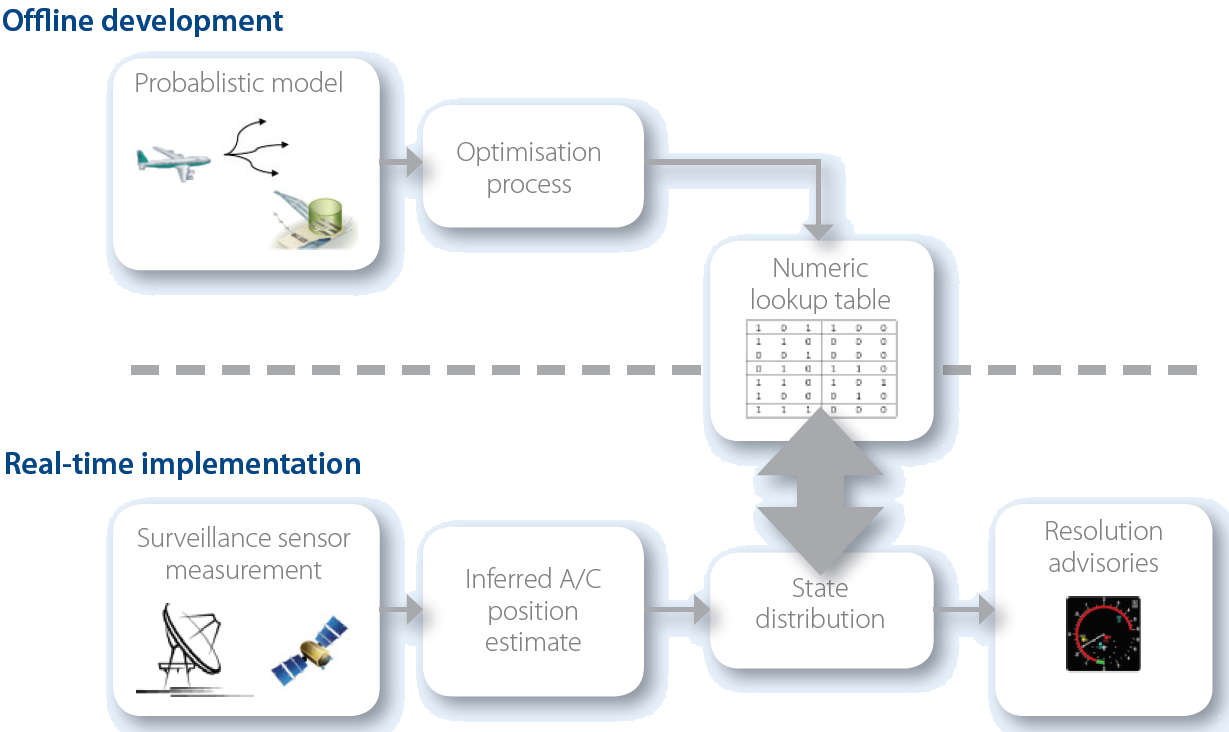
\includegraphics[width=.8\linewidth]{\FIGDIR/TE058TwoPhasesACASX}
    \caption{ACAS-X concept scheme \cite{netalert2013n17}.}
    \label{fig:acasxConceptScheme}
\end{figure}

\begin{note}
    \emph{Two-phase calculation} with offline development and real-time operation phase concept, will be used in different manner in our method. (sec. \ref{s:avoidanceConcept})
\end{note}

\paragraph{Advisories:} The \emph{ACAS-X} is taking the advisories categorization from \emph{ICAO Annex 10.} \cite{annex200710}. The advisories are recommended (directives for UAS) actions to take.


Airborne Collision Avoidance Systems (ACAS) equipment provides two types of advisories to pilots: Resolution Advisories (RAs) and Traffic Advisories (TAs). These are defined as follows:

\begin{enumerate}
    
    \item \emph{Resolution advisory} (RA) - an indication given to the flight crew recommending:
    
    \begin{enumerate}[a.]
        \item Manoeuvre intended to provide separation from all threats.
        
        \item Manoeuvre restriction intended to maintain existing separation.
    \end{enumerate}
    
    \item \emph{Corrective resolution advisory} - a resolution advisory that advises the pilot to deviate from the current flight path.
    
    \item \emph{Preventive resulution advisory} - a resolution advisory that advises the pilot to avoid certain deviations from the current flight path but does not require any change in the current flight path.

    \item \emph{Traffic advisory} (TA) - An indication given to the flight crew that a certain intruder is a potential threat.
\end{enumerate}

\begin{note}
    The \emph{UAS} system with full autonomy must handle the solution of the \emph{directives} (advisories) form UTM and other systems. The example of configurable handling mechanism - \emph{Rule engine} is given in (sec. \ref{s:RuleEngineArchitecture}).
\end{note}

\paragraph{Example Overview of the Incident:} The \emph{example of incident} and  a resolution is outlined in (fig. \ref{fig:axasxincidentoverviewexample}). The \emph{example} is given for better understanding of \emph{ACAS-X} roles \& responsibilities. 

\begin{itemize}
    \item[1.] \emph{Initial state} - the initial state is given like follow:
    
    \emph{Green Airplane} (A/C 1) is cruising on \emph{flight level} FL-390 (39 000 feet)
    
    \emph{Orange Airplane} (A/C 2) is cruising on \emph{flight level} FL-370 (37 000 feet)
    
    \item[2.] \emph{Orange aircraft transponder mishap} - the \emph{orange airplane} appears on flight level FL-405 (45 000 feet).  The \emph{green aircraft} controller (pilot) wants to \emph{descent} to oragne aircraft real flight level (FL-370). 
    
    \item[3.] \emph{Green airplane descent} - the \emph{Green aircraft} starts to descent. The \emph{Orange aircraft} keeps the flight level (FL-370). 
    
    \item[4.] \emph{Green aircraft Active Surveillance} - the \emph{green aircraft} uses \emph{active surveillance} to detect \emph{orange aircraft}. 
    
    The \emph{ACAS-X} issues \emph{Adjust Vertical Speed, Adjust - Resolution Advisory} (AVSA RA) to  the \emph{green aircraft} to \emph{level off} and stop \emph{descent} or at least slow it.
    
    Then as \emph{ACAS-X} issues \emph{Climb Resolution Advisory} to the \emph{green aircraft} mandating to get altitude. 
    
    \begin{note}
        The main issue is that \emph{pilot} is responsible decision maker, therefore pilot can refuse to follow \emph{ACAS-X advisories}.
    \end{note}
    
    \item[5.] \emph{Orange airplane starts descending} -  the \emph{orange aircraft} detects the \emph{flight level disparity} due the \emph{active surveliance} deteciton of \emph{green aircraft} on \emph{FL-370}.
    
    The \emph{Green aircraft} is tail-gating \emph{orange aircraft} from above. The \emph{ACAS-X} evaluates situation and issues a \emph{Descent Resolution Advisory} to avoid pursuit. 
    
    The \emph{pilot} of \emph{orange aircraft} follows the order of RA
\end{itemize}


\begin{figure}[H]
    \centering
    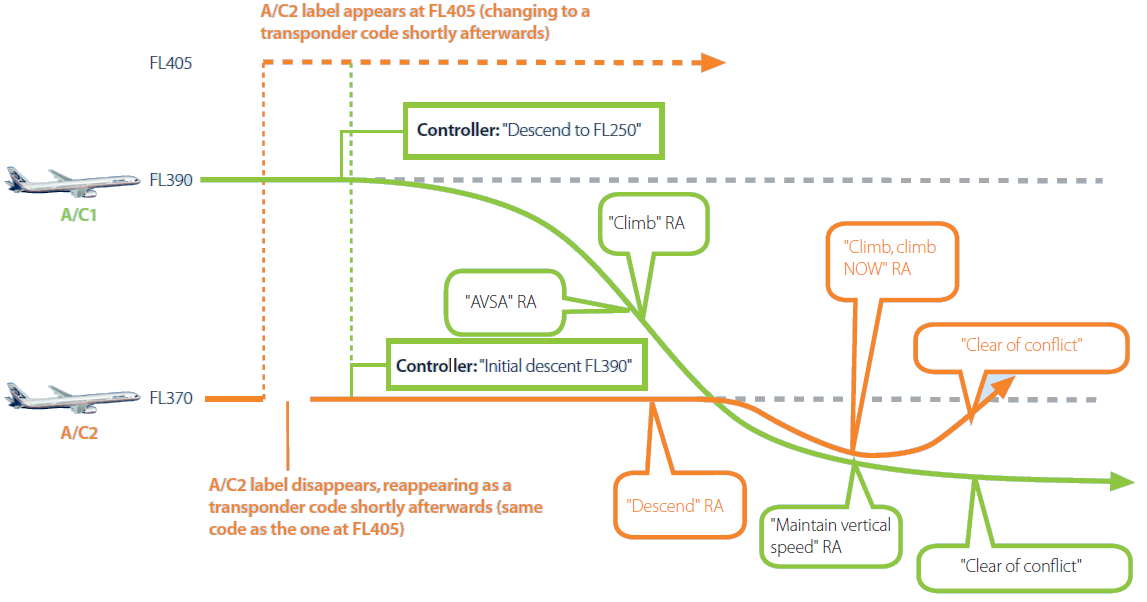
\includegraphics[width=\linewidth]{\FIGDIR/TE059ACASConflictExample}
    \caption{ACAS-X incident overview \cite{netalert2013n17}.}
    \label{fig:axasxincidentoverviewexample}
\end{figure}

\begin{itemize}
    \item[6.] \emph{Tailgating detection} - the \emph{orange airplane} is in front of \emph{green airplane}, both airplanes are descending at same rate. 
    
    \begin{note}
        This situation is very dangerous, because it is very close to \emph{intentional pursuit scenario}.
    \end{note}
    
    The \emph{orange airplane} is \emph{pursued}, its own \emph{ACAS-X} issues the \emph{Climb Now Resolution Advisory}. The pilot follows the advisory.
    
    The \emph{green airplane} is \emph{pursuing} and its goal is to \emph{descent} to flight level FL-250. Its \emph{ACAS-X} issues \emph{maintain vertical speed resolution advisory}.
    
    \item[7.] \emph{Conflict resolution} - both airplanes follow \emph{Resolution Advisories}.  When significant vertical distance is reached. The conflict is marked as resolved. 
\end{itemize}

